\chapter{Results and Discussion}
\label{chap:evaluation}

The implemented prototype shows that it is possible to get structured data out of the stenographic transcripts and that analysis can be performed on the basis of this data. The analysis can give an overview of politician absence, length of serving in the national council, politician activity, the relation between politicians/clubs and the inner cohesion of coalition or opposition. A web application was developed which shows the results and makes them accessible for everybody. Figure \ref{fig:start_page_prototype} shows the start page of this application.

\begin{figure}[h]
	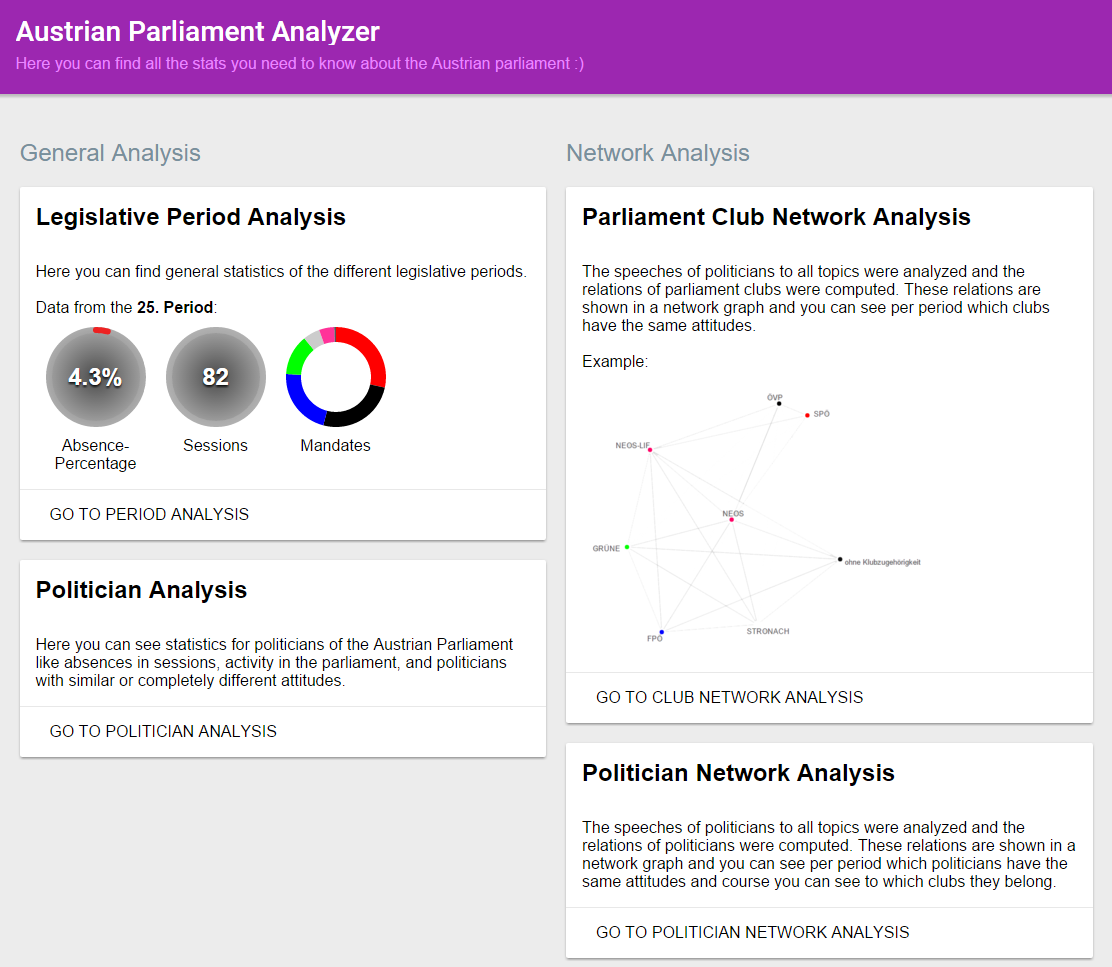
\includegraphics[width=\textwidth]{imgs/result_start_page}
	\caption{Start Page of the Prototype Web Application}
	\label{fig:start_page_prototype}
\end{figure}

\section{Relations of Parliament Clubs}
\label{sec:relations_clubs}

\begin{figure}
\begin{tabular}{ l r }
	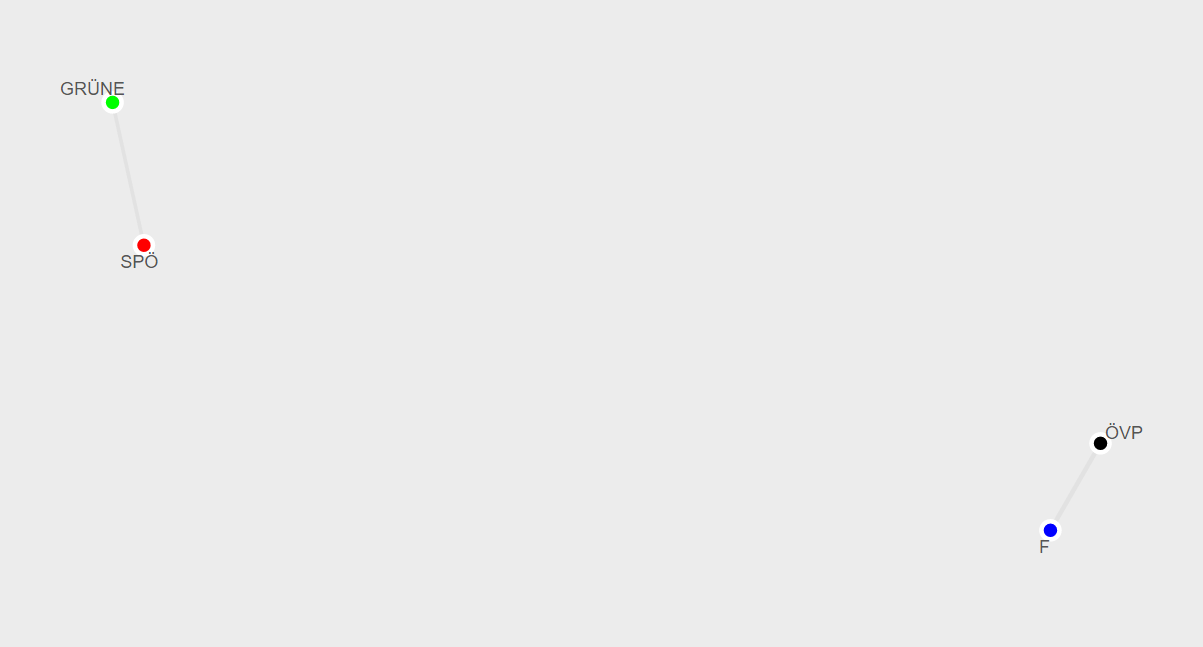
\includegraphics[width=0.49\textwidth]{imgs/graphs/club-graphs/clubs_21} & 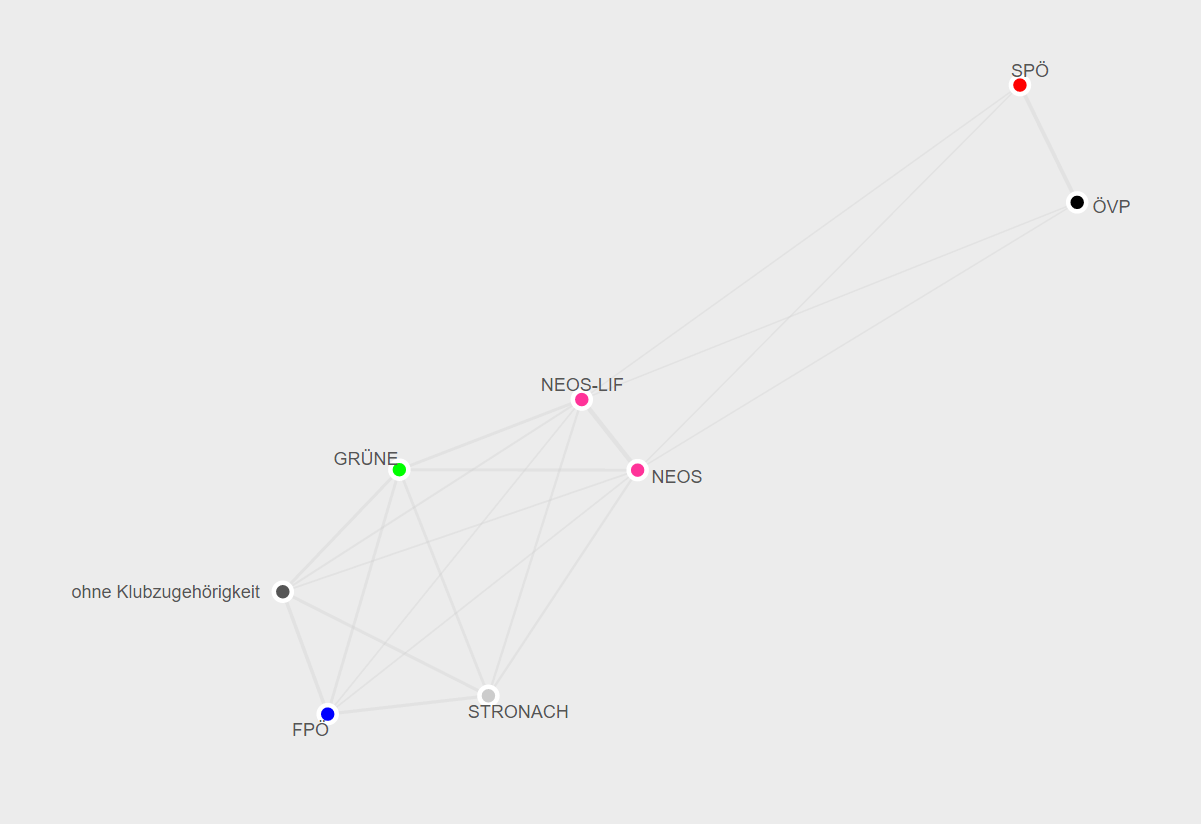
\includegraphics[width=0.49\textwidth]{imgs/graphs/club-graphs/clubs_25}
\end{tabular}
	\caption{Club ............}
	\label{fig:club_graphs1}
\end{figure}


\section{Relations of Politicians}
Graph + Explanations

\section{Government - Opposition Relation}
\label{sec:gov_opp_relation}

asdf

\begin{table}[h]

\centering
\bgroup
\def\arraystretch{1.2}
\begin{tabular}{| p{4cm} | p{3cm} | l |}
\hline
  Legislative Period & Governing Parties & Opposition  \\
\hline
\hline
  20. Period: 1995 - 1999 & SPÖ, ÖVP & FPÖ, Grüne, Liberale \\
\hline
  21. Period: 1999 - 2002 & ÖVP, FPÖ & SPÖ, Grüne \\
\hline
  22. Period: 2002 - 2006 & ÖVP, FPÖ, BZÖ\footnote{The BZÖ was in government from $17^{th}$ of April, 2005} & SPÖ, Grüne \\
\hline
  23. Period: 2006 - 2008 & SPÖ, ÖVP & FPÖ, Grüne, BZÖ \\
\hline
  24. Period: 2008 - 2013 & SPÖ, ÖVP & FPÖ, Grüne, Stronach, BZÖ \\
\hline
  25. Period: since 2013 & SPÖ, ÖVP & FPÖ, Grüne, NEOS, Stronach \\
\hline

\end{tabular}
\egroup
\caption{Government and Opposition in the Legislative Periods 20 to 25}
\label{table:gov_opp_parties}
\end{table}



\begin{table}[h]

\centering
\bgroup
\def\arraystretch{1.2}
\begin{tabular}{| p{2cm} | p{3cm} | p{3cm} | p{3cm} |}
\hline
  Legislative Period & Government-Opposition Relation & Inner Government Relation & Inner Opposition Relation \\
\hline
\hline
  20. Period & -0.85 & +1.00 & +0.86 \\
\hline
  21. Period & -0.695 & +0.985 & +0.908 \\
\hline
  22. Period & -0.567 & +1.00 & +0.938 \\
\hline
  23. Period & -0.382 & +0.994 & +0.765\\
\hline
  24. Period & -0.52 & +1.00 & +0.768\\
\hline
  25. Period & -0.374 & +1.00 & +0.676\\
\hline

\end{tabular}
\egroup
\caption{Government-Opposition Relation, Inner Government- and Inner Opposition Relation for the Legislative Periods 20 to 25}
\label{table:gov_opp_relation}
\end{table}